\section{Results}\label{sec:results}
\subsection{Proving and Verifying Times}\label{subsec:results:provingverifying}

After running the experiment comparing Curdleproofs and CAAUrdleproofs across different shuffle sizes, we obtained the results shown in \autoref{fig:resulttimes}.

\begin{figure*}[!htb]
    \centering
    \subfloat[\centering Proving Time]{{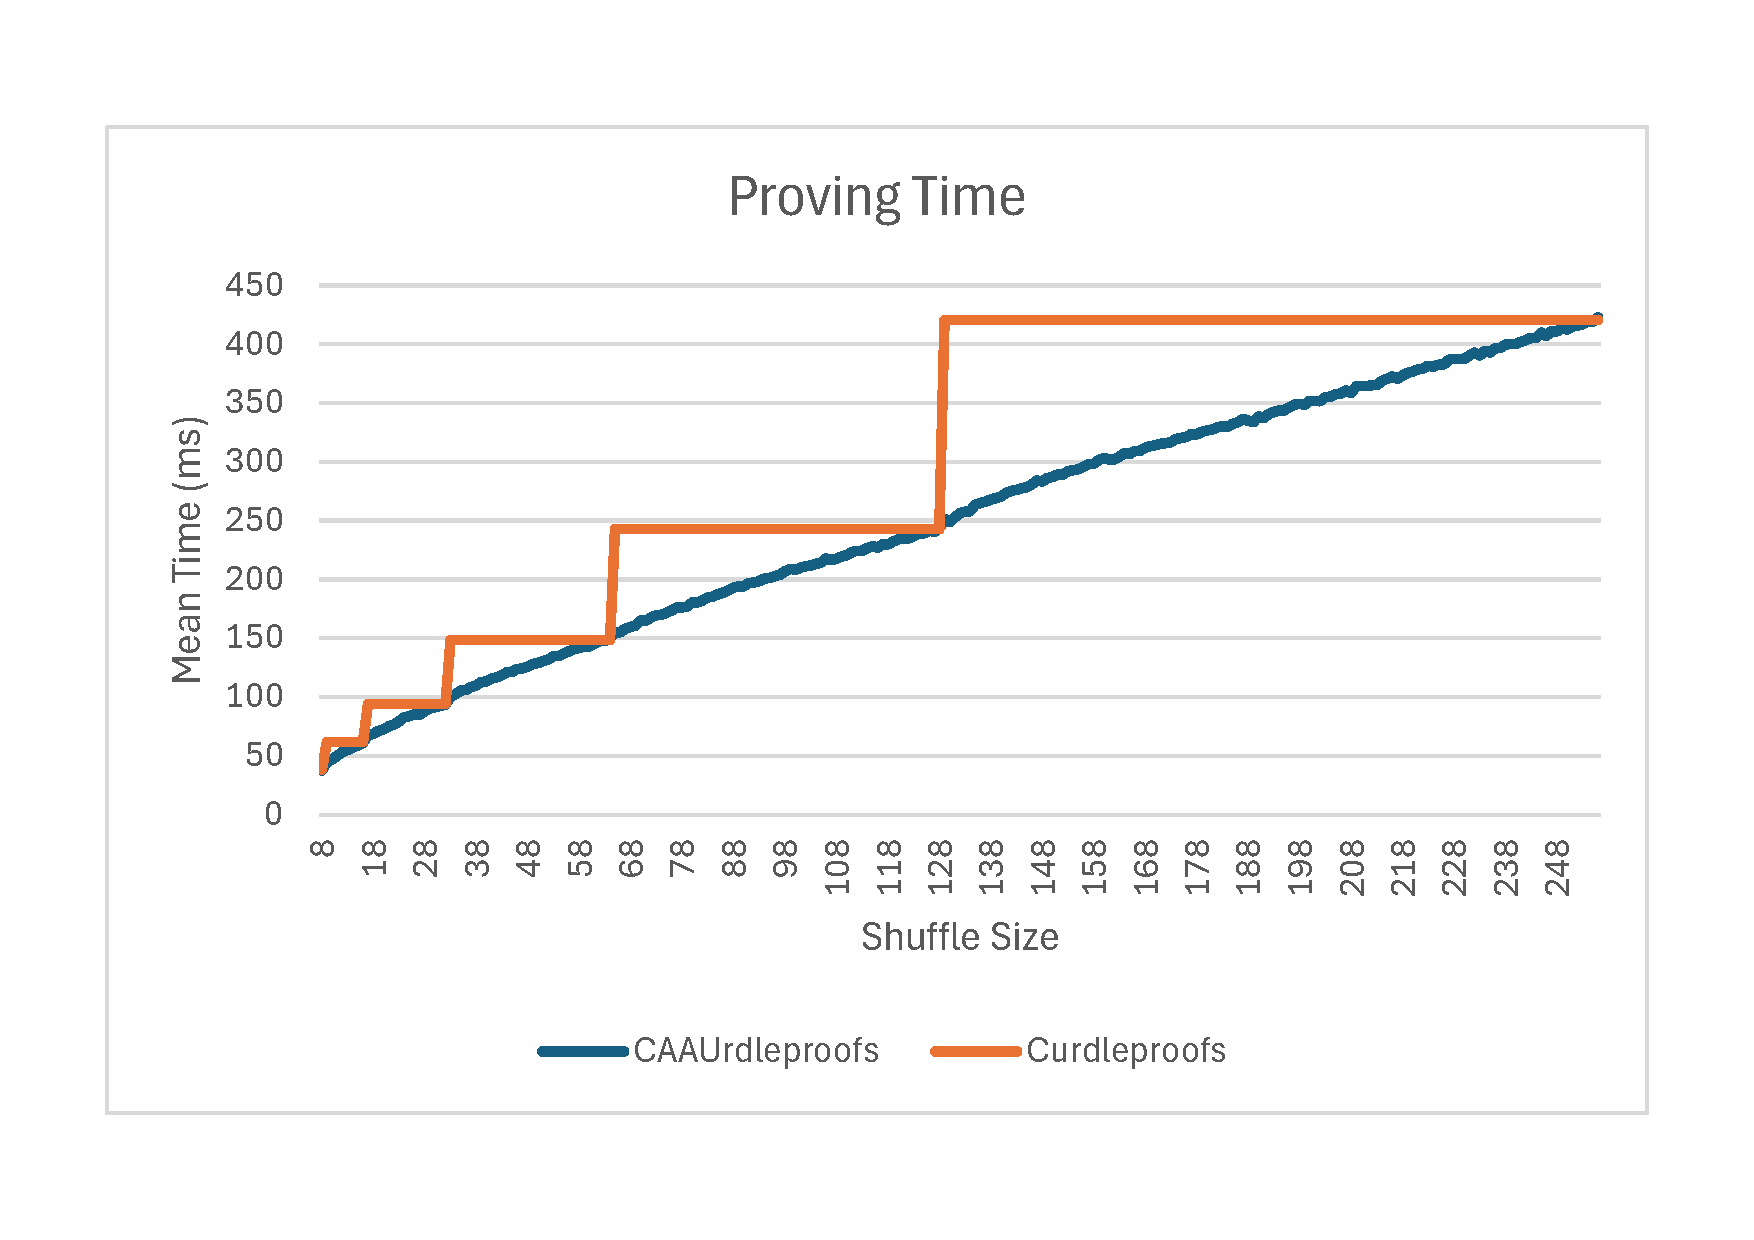
\includegraphics[width=0.47\textwidth]{figures/results/provingtime} }}%
    \qquad
    \subfloat[\centering Verifying Time]{{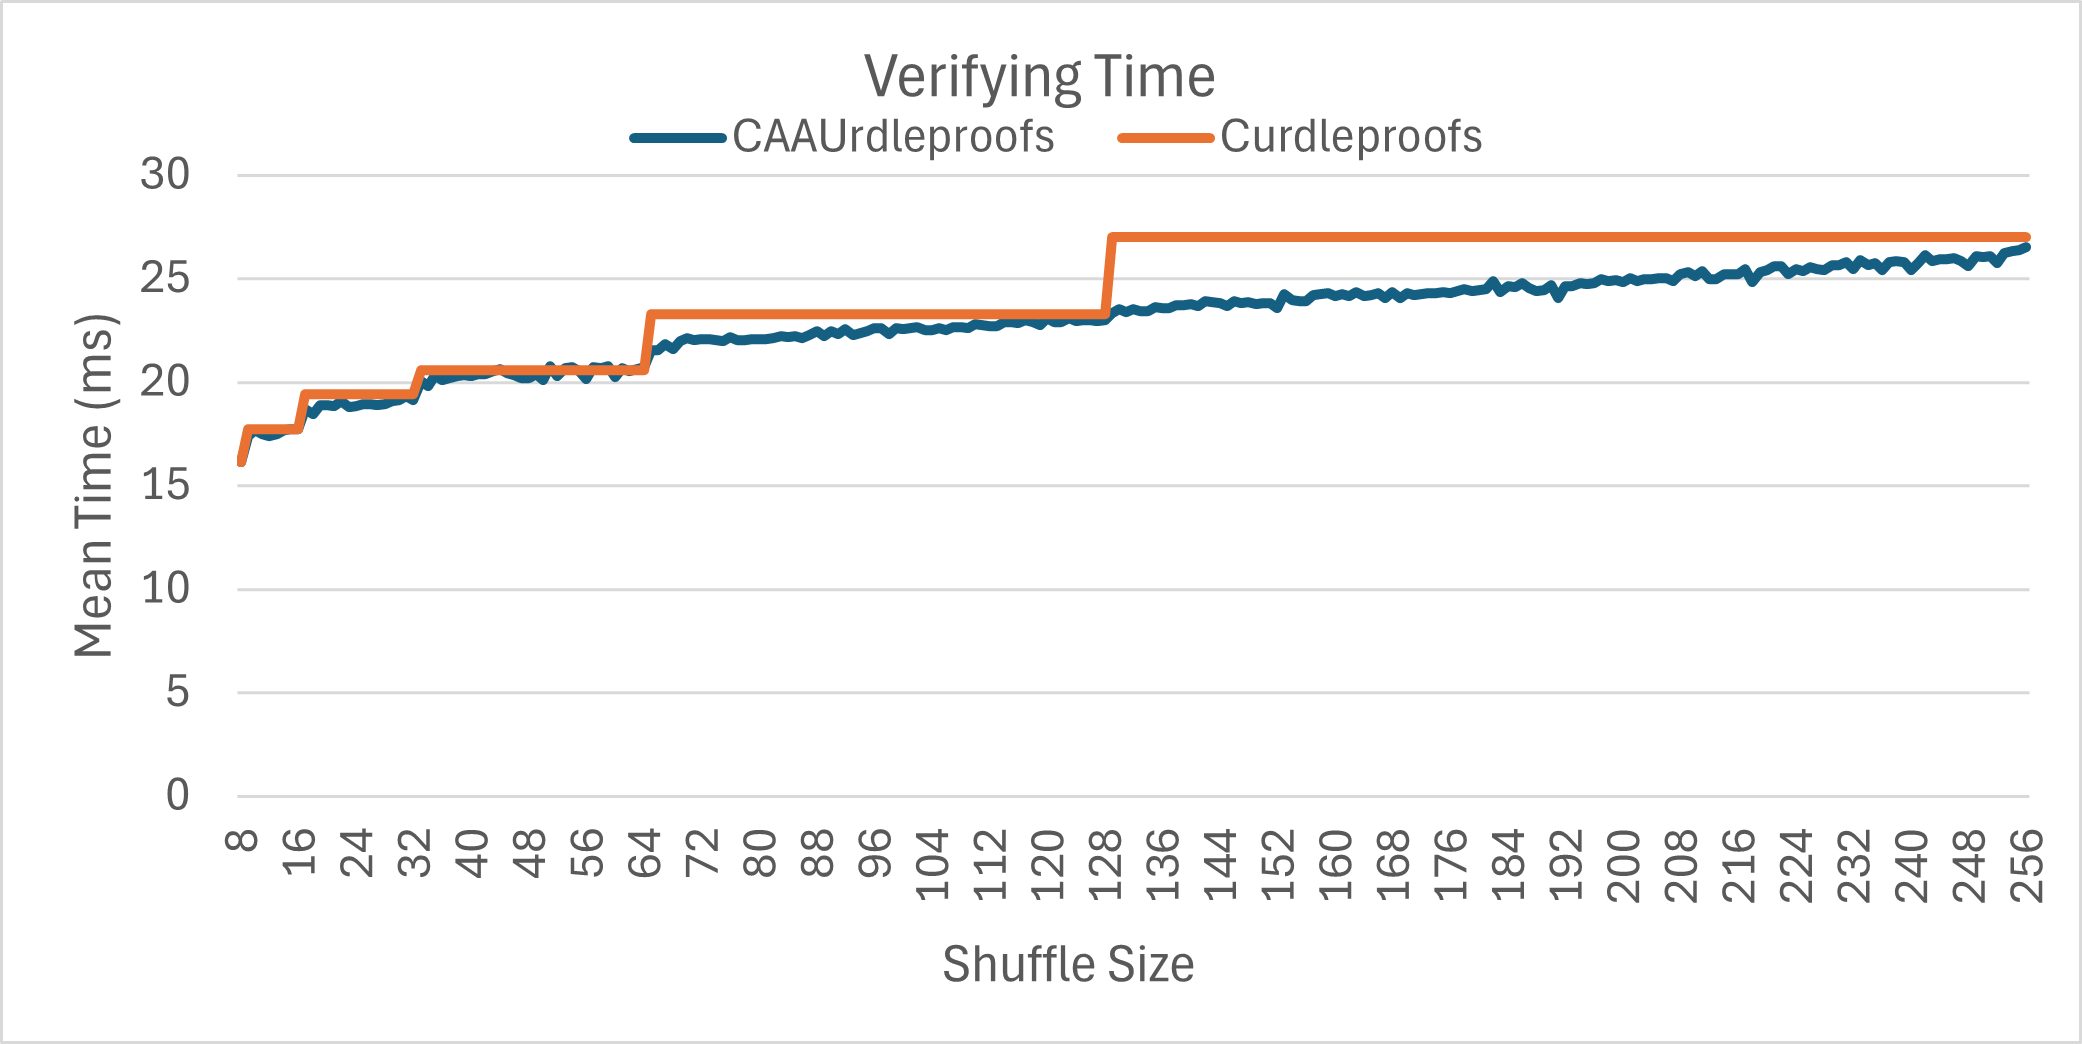
\includegraphics[width=0.47\textwidth]{figures/results/verifyingtime} }}%
    \caption{The timed results compared between CAAUrdleProofs and Curdleproofs}%
    \label{fig:resulttimes}%
\end{figure*}

As mentioned in \autoref{sec:CAAUrdleproof-experiment}, CAAUrdleproofs was run with a shuffle size $\ell=\{8,9,\dots,256\}$.
Curdleproofs was only run with a shuffle size $\ell = 2^N$, where $N = \{3,4,5,6,7,8\}$, as it is only able to run in powers of two.
Hence, the results for Curdleproofs show that the shuffle size,~$\ell$, instantly increases to the next power of two because it theoretically would have to pad the input set until it reaches the next power of two.

From the results, we can see that CAAUrdleproofs and Curdleproofs have similar proving and verifying times when~$\ell$ is a power of two.
However, when~$\ell$ is not a power of two, CAAUrdleproofs is faster.
When~$\ell$ is below a power of two, we observe that the performance advantage of CAAUrdleproofs over Curdleproofs increases as~$\ell$ decreases.

The results for the verifying time also show that the verifying time jumps up quite significantly the first four times it reaches above a power of two.
However, this is not the case, at least not as aggressively, when increasing $\ell$ from 128.
We find, however, that the bump is smaller the higher $\ell$ is.

In addition to the proving and verifying times, the time used on shuffling is also lower for any $\ell$ that is not a power of two; see Appendix~\ref{sec:shuffling-results}.
However, that was to be expected since CAAUrdleproofs uses the same shuffling algorithm as Curdleproofs but does not have to add additional padding to the non-power of two input sizes.



\subsection{Shuffle Security}\label{subsec:Shuffle-security}

\begin{figure}[!htb]
    \centering
    \subfloat[\centering]{{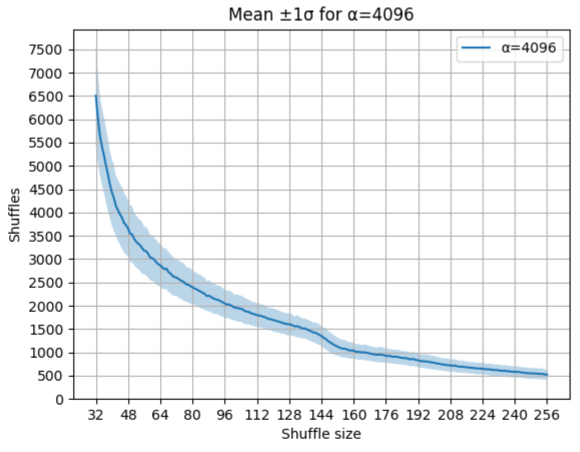
\includegraphics[width=0.99\columnwidth]{figures/results/4096-256-p2}}}\\[-2pt]
    \subfloat[\centering]{{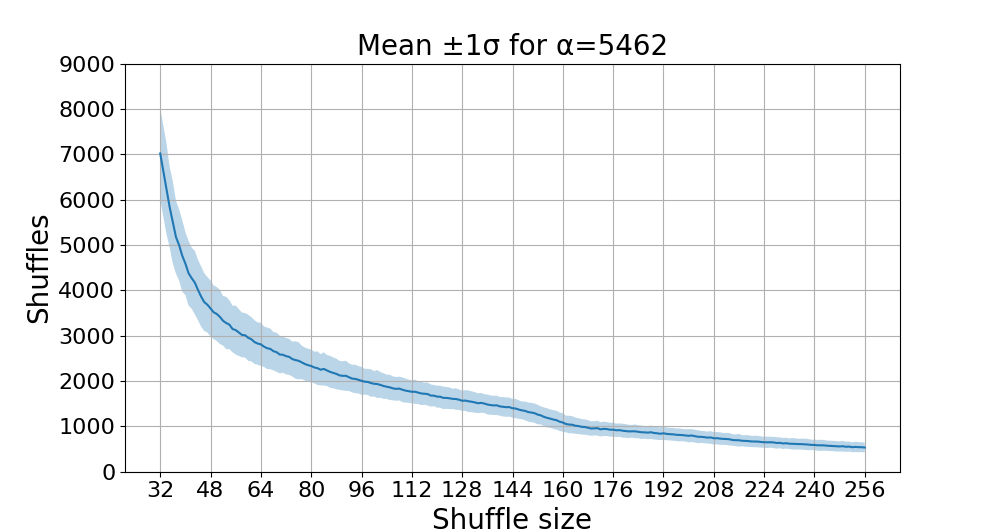
\includegraphics[width=0.99\columnwidth]{figures/results/5462-256-p2}}}\\[-2pt]
    \subfloat[\centering]{{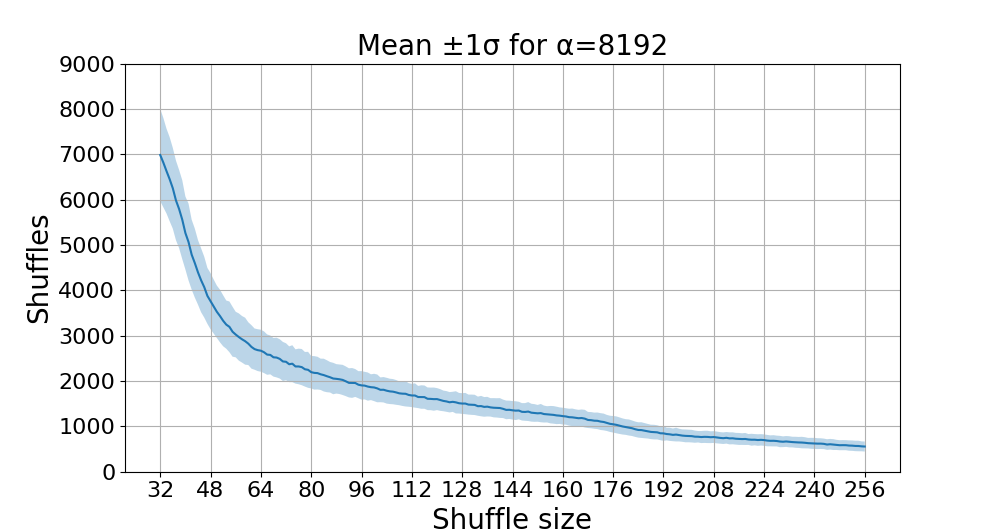
\includegraphics[width=0.99\columnwidth]{figures/results/8192-256-p2}}}\\[-2pt]
    \caption{Results of shuffle security experiment showing mean amount of honest shuffles necessary with one standard deviation}%
    \label{fig:shufflesecurity}%
\end{figure}

\begin{figure}[!htb]
    \centering
    \subfloat[\centering]{{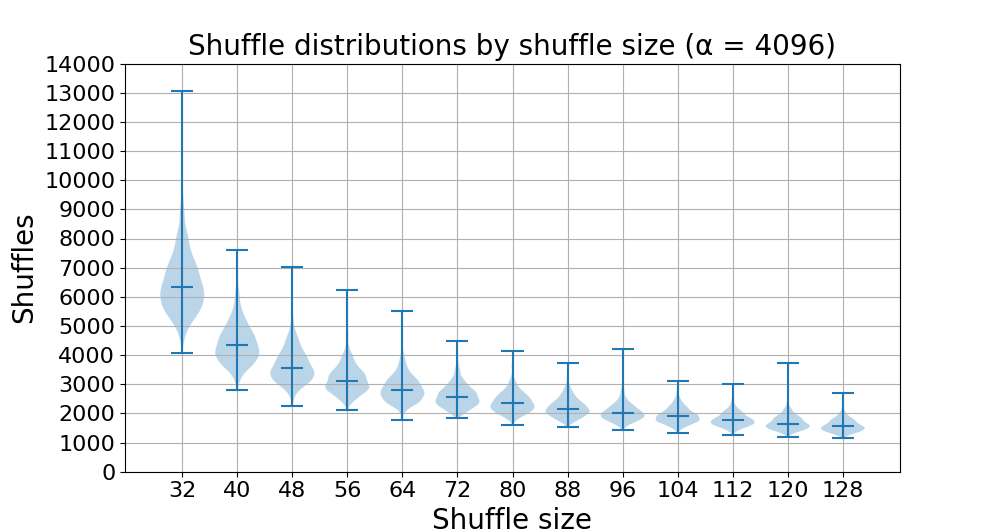
\includegraphics[width=0.99\columnwidth]{figures/results/violin-4096}}}\\[-2pt]
    \subfloat[\centering]{{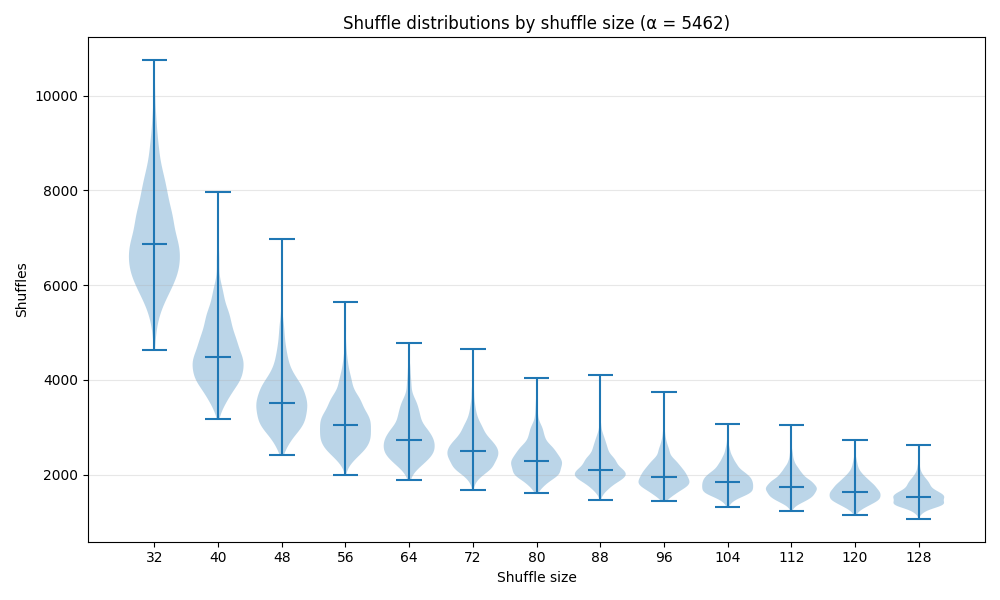
\includegraphics[width=0.99\columnwidth]{figures/results/violin-5462}}}\\[-2pt]
    \subfloat[\centering]{{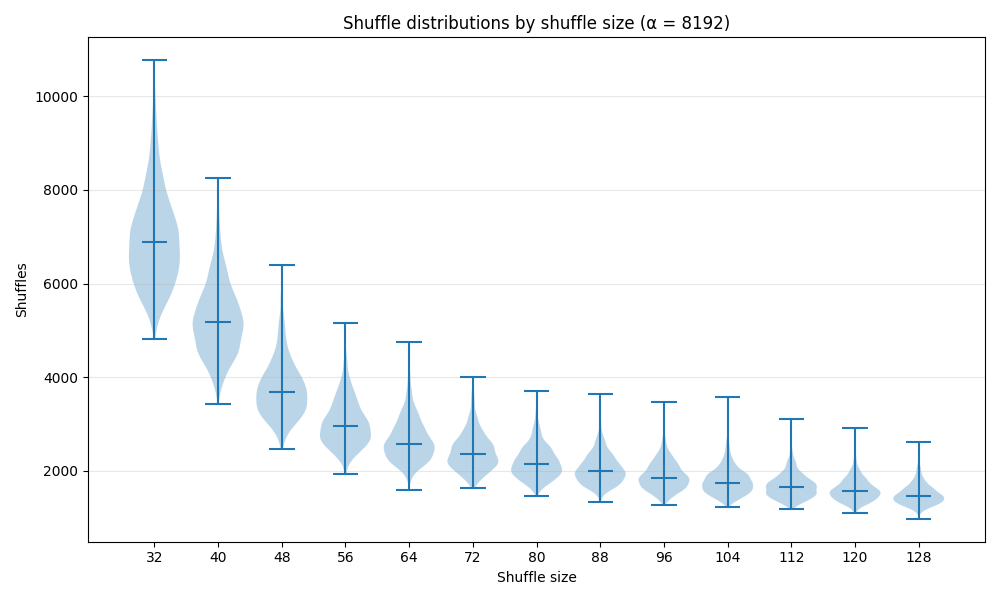
\includegraphics[width=0.99\columnwidth]{figures/results/violin-8192}}}\\[-2pt]
    \caption{Results of shuffle security experiment showing spread of nessecary shuffles needed for shuffle to be secure}%
    \label{fig:shufflesecurityviolin}%
\end{figure}

The results of the shuffle security experiment are shown in \autoref{fig:shufflesecurity}.

\autoref{fig:shufflesecurity} shows the mean of the 1,000 runs of each shuffle size $\ell$ and the standard deviation.

We can see that the bigger the shuffle size $\ell$ is, the less honest shuffles are necessary to make the shuffle secure.
In Ethereum, each shuffling phase is limited to 8,192 shuffles, meaning that the maximum number of honest shuffles that can be used is 8,192.
Therefore, the results of the experiment find $Q_H=Q-\beta$.
$Q_H$~is how many of the $Q$ shuffles available during the shuffling phase are needed to be honest.
The rest is, therefore, the maximum number of dishonest shuffles allowed,~$\beta$.
We also see that the bigger the shuffle size, the narrower the standard deviation gets.

From the results of the experiment, with~$\alpha=8,192$, we can see that the number of honest shuffles necessary to make the shuffle secure sharply decreases until the size of $\ell=64$, and then it starts to level out.
We can see that with a size of $\ell=75$, we need about 1/3 of the shuffles to be honest to make the shuffle secure.
Likewise, we see that, at~$\ell=108$, we need about 1/4 of the shuffles to be honest to make the shuffle secure.

In general, all three of the experiments, despite the difference in $\alpha$, show the same trend.
They all level out, but the higher~$\alpha$ is, the lower the leveling occurs, and the later it happens as well.
There are two things, however, that are different between the experiments.
At~$\alpha=4,096$, we see that with $\ell=32$, the mean number of honest shuffles necessary to make the shuffle secure is $\sim500$ lower than the two other $\alpha$ values.
As~$\ell$ increases, the mean number of honest shuffles necessary to make the shuffle secure becomes similar to the other $\alpha$ values.
Another thing that differs between the experiments is that they all have a sudden dip in higher $\ell$ values in the experiment.
Here, we observe a trend that the lower the~$\alpha$ is, the earlier the dip occurs.



The results in \autoref{fig:shufflesecurityviolin} show that for all three $\alpha$ values, the spread of the necessary honest shuffles tightens the larger the shuffle size $\ell$ gets.
Like the results in \autoref{fig:shufflesecurity}, \autoref{fig:shufflesecurityviolin} also shows that the bigger a shuffle size $\ell$, the less honest shuffles, on average, are necessary to make the shuffle secure.

We can also see that the widest point of the violin plot is below the mean, meaning the outliers are a lot more significant above the mean than below it.

It is worth noting that there is a spike in the distribution of the necessary honest shuffles at $\ell=32$ for $\alpha=4,096$.
This spike is not present for the other two $\alpha$ values and is likely due to the probabilistic nature of the shuffling method.

Another notable aspect is that in the Ethereum setting, the maximum number of shuffles available is 8,192.
Therefore, in the cases where more than the 8,192 shuffles were necessary to make the shuffle secure, the shuffle would not have been secure within the Ethereum setting.
Hence, it is also possible to see the experiment as running 1,000 days worth of each shuffle size $\ell$ and then seeing how many of those days would have been secure.
We found that the first size of $\ell$ that could have been secure for the entire duration of the experiment would be $\ell=42$ for $\alpha=8,192$ and $\ell=40$ for $\alpha=5,462$ and $\alpha=4,096$.


